\begin{surferPage}{En dobbel kjegle}
 Som vi forklarte i introduksjonen til galleriet, er en flate glatt dersom den ikke har noen 
 toppunkter (slike punkter kalles singulariteter). For eksempel gjelder det en kule eller
 en torus (de to bildene til venstre under):

    \begin{center}
      \vspace{-0.3cm}
      \begin{tabular}{@{}c@{}c@{}c@{}c@{}}
        \begin{tabular}{@{}c}
          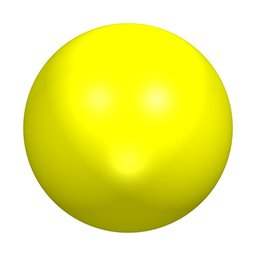
\includegraphics[width=1.4cm]{./../../common/images/kugel}
        \end{tabular}
        &
        \begin{tabular}{@{}c}
          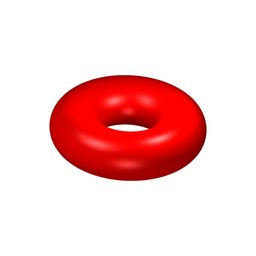
\includegraphics[width=1.4cm]{./../../common/images/torus}
        \end{tabular}
        &
        \begin{tabular}{c@{}}
          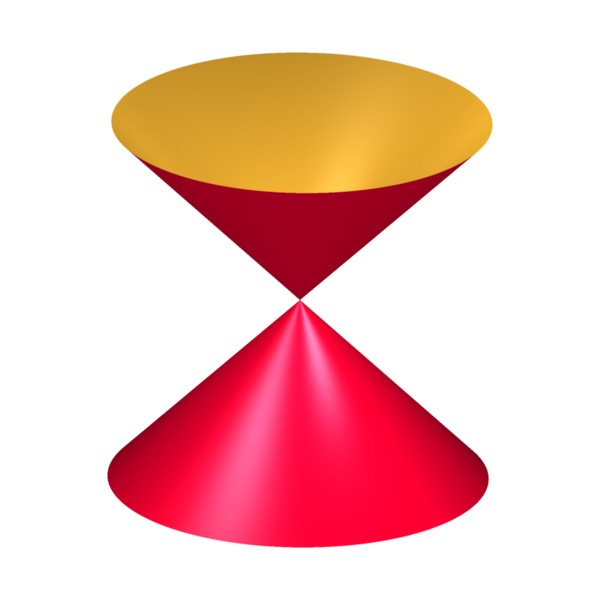
\includegraphics[width=1.4cm]{./../../common/images/kegel}
        \end{tabular}
      \end{tabular}
    \end{center}
    \vspace{-0.3cm}
    Den doble kjeglen (bildet lengst til høyre) er den enkleste singulariteten og den eneste som kan beskrives av en andregradsligning:
    \[x^2+y^2-z^2=0.\]
	
	Hvis denne ligningen endres litt ved å erstatte $0$ med en liten verdi $a\neq 0$, 
	omformes den doble kjeglen til en av de to typene av hyperboloider, avhengig av fortegnet til $a$:
	
%    \dontshow{
    % 
    \begin{center}
      \vspace{-0.2cm}
      \begin{tabular}{@{}c@{\ }c@{\ }c@{\ }c@{\ }c@{}}
        \begin{tabular}{@{}c@{}}
          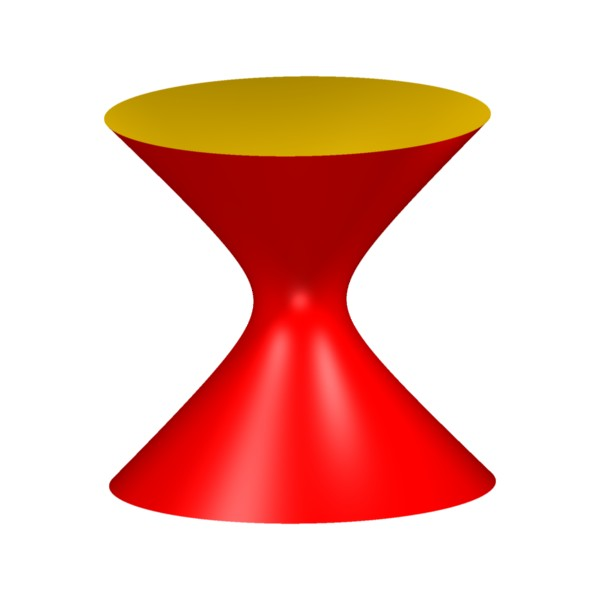
\includegraphics[width=1.2cm]{./../../common/images/A1pm_2}
        \end{tabular}
        &
        $\leftarrow$
        &
        \begin{tabular}{@{}c@{}}
          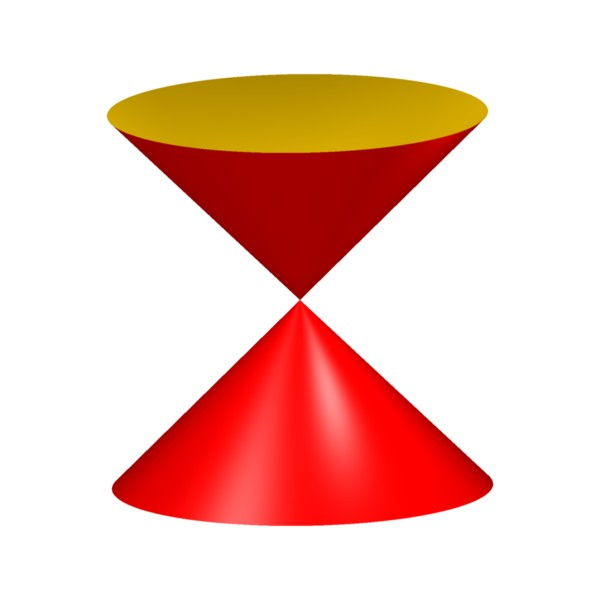
\includegraphics[width=1.2cm]{./../../common/images/A1pm_1} 
        \end{tabular}
        &
        $\rightarrow$
        &
        \begin{tabular}{@{}c@{}}
          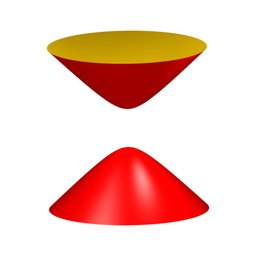
\includegraphics[width=1.2cm]{./../../common/images/A1pm_0}
        \end{tabular}
      \end{tabular}
    \end{center}
%    }
    \vspace{-0.2cm}
   En flate av andre grad kan ikke ha mer enn én singularitet, det vil si at\  
    $\mu(2)=1$.
\end{surferPage}
